\documentclass[compress]{beamer}
\usetheme{Warsaw}

\mode<presentation>

\title{Bayesian Phase Unwrapping with Factor Graphs}
\subtitle[6.556]{6.556 Final Project}
\author{Eric Jonas}
\date{May 12, 2009}
\institute[MIT BCS]{MIT Brain \& Cognitive Sciences}

\begin{document}

\begin{frame}
\maketitle
\includegraphics{4node_fg}
\end{frame}

\begin{frame}
\tableofcontents
\end{frame}

\section{Phase Unwrapping for MR}
\frame{\tableofcontents[currentsection]}

\begin{frame}
  \frametitle{Phase Unwrapping for MR} 
    \begin{columns}
    \begin{column}{6cm}
      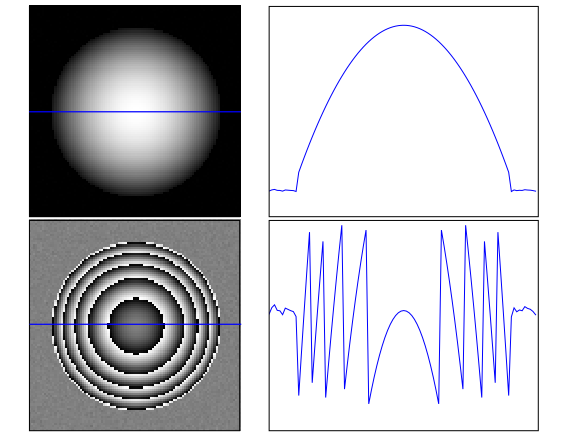
\includegraphics[width=6cm]{phase_wrap_example.pdf}

    \end{column}
    \begin{column}{5cm}
      We think phase information varies smoothly except at boundaries

      Right now most clinical applications only focus on magnitude

      Phase provides additional information, such as field inhomogeneity
      and fluid velocity
      \pause
      \begin{alertblock}{Phase Wrapping}
        Our phase observations map $(-\infty, \infty)$ to $(0, 2\pi)$
      \end{alertblock}
    \end{column}
  \end{columns}

\end{frame}

\section{MRFs and Factor Graphs}
\frame{\tableofcontents[currentsection]}
\begin{frame}
  \frametitle{Markov Random Fields}
  \begin{columns}
    \begin{column}{5cm}
      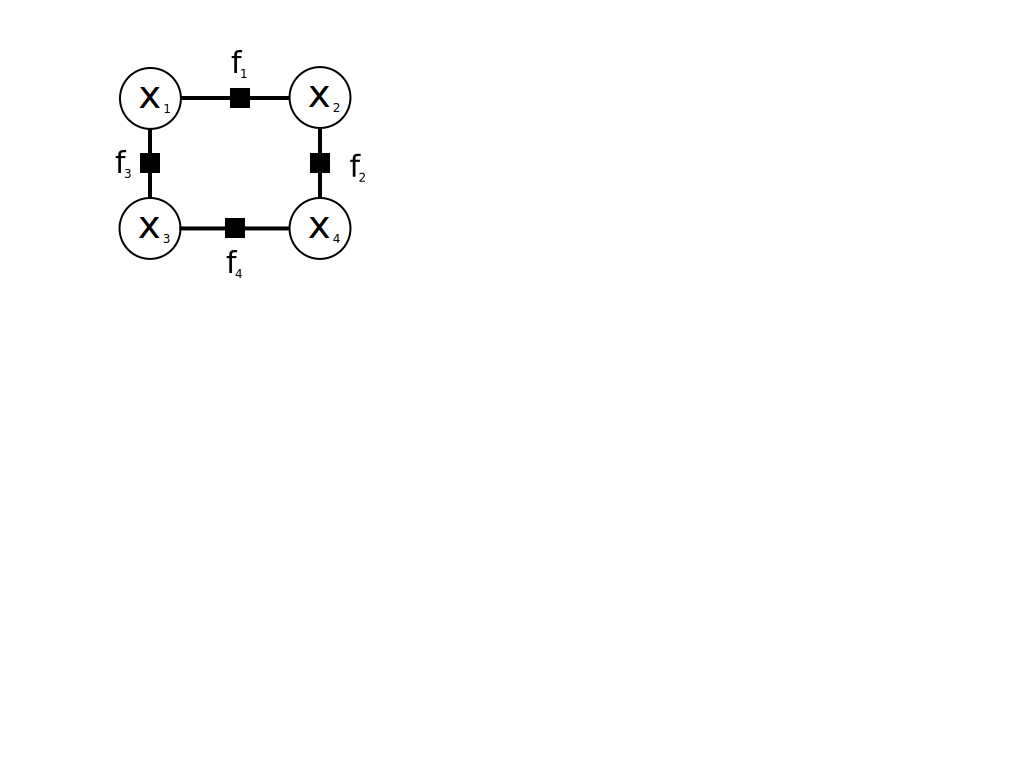
\includegraphics[width=5cm]{4node_mrf.pdf}
    \end{column}
    \begin{column}{5cm}
      \begin{itemize}
        \item You may know as ``Undirected graphical model'' 
        \item Each $X_i$ is a variable, we'll call it ``state'' 
          \item Implicitly we know a series of joint distributions on the $x_i$ represented by edges
        \end{itemize}
    \end{column}
  \end{columns}
\end{frame}

\begin{frame}
  \frametitle{Factor Graphs}
  \begin{columns}
    \begin{column}{5cm}
      \includegraphics[width=4cm]{4node_fg.pdf}
    \end{column}
    \begin{column}{5cm}
      \begin{itemize}
        \item Factor Graphs \cite{kschischang_factor_2001} express the same concepts
          as MRFs but make the \textbf{factors} explicit. 
        \end{itemize}
    \end{column}
  \end{columns}
  \begin{block}{Factor Graph Probability}
    $P(x_1, x_2, x_3, x_4) = f_1(x_1, x_2) \cdot f_2(x_2, x_3) \cdot f_3(x_3, x_4) \cdot f_4(x_4, x_1)$
  \end{block}
\end{frame}

\begin{frame}
  \frametitle{Example : Ising Model}
  Imagine you want to simulate a spin system
  Statistical physics people love doing this

\end{frame}


\begin{frame} 
  \frametitle{Factor Graphs for Low-Level Vision}
  \begin{columns}
    \begin{column}{5cm}
      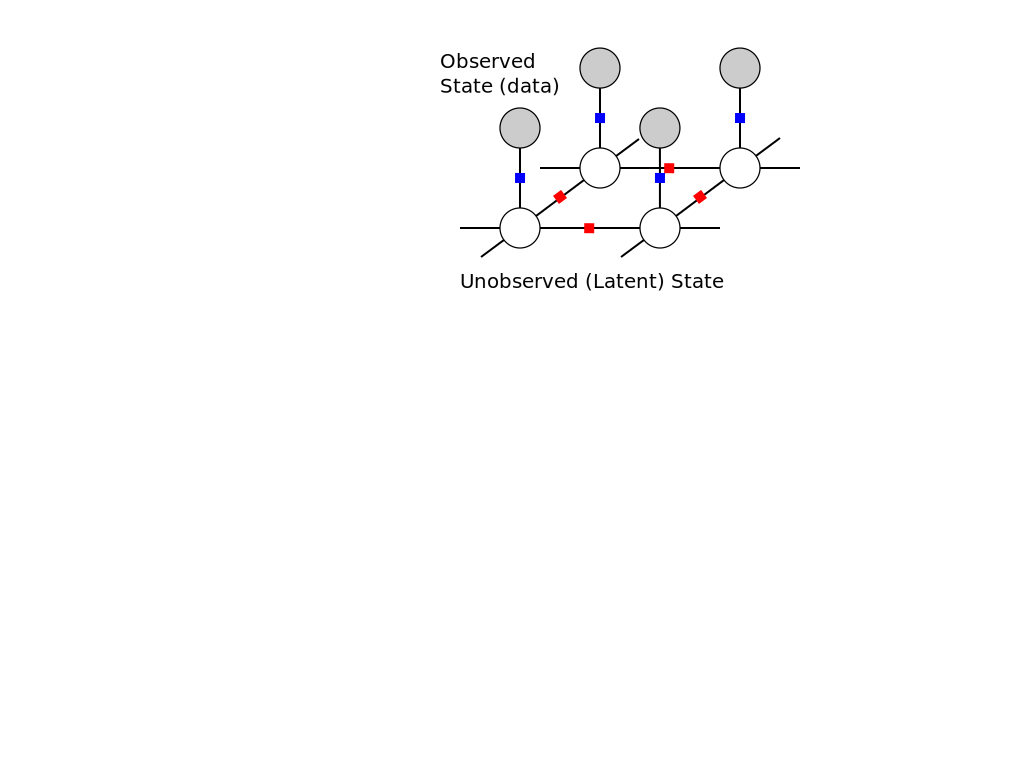
\includegraphics[width=6cm]{image_fg.pdf}
    \end{column}
    \begin{column}{5cm}
      Properties of Image Factor Graphs \cite{Freeman_Markov_1999}: 
      \begin{itemize}
      \item Use observed state (data) to infer hidden state
      \item Have lattice structure like the ising
      \item Large number of vertices ($O(n)$ in number of pixels)
      \item $O(1)$ per-vertex connectivity
      \item Typically have homogeneous factors
      \end{itemize}
    \end{column}
  \end{columns}
\end{frame}

\begin{frame}
\frametitle{Bayesian Factor Graphs}
\begin {columns}
  \begin{column}{5cm}
    \begin{block}{Bayes Rule} 
      \begin{equation*}
        P(X | Y ) = \frac{P(Y | X) P(X)}{\sum_XP(Y|X)P(X)}
      \end{equation*}
    \end{block}
  \end{column}
  \begin{column}{5cm}
    \begin{itemize}
    \item $Y = {y_{(i, j)}}$ : Observed Nodes
    \item $X = {x_{(bi, j)}}$ : Hidden state we wish to estimate
    \item $P(Y | X) $ : measurement model (``likelihood'')
    \item $P(X) $ : prior 

    \end{itemize}
  \end{column}
  
  \end{columns}
\end{frame}

\begin{frame}
\frametitle{Bayesian Factor Graphs For Low-Level vision}
Our factor graph gives us P(X, Y), we want $P(X | Y)$. 

\begin{block}{Bayes Rule} 
  \begin{equation*}
    P(X | Y ) = \frac{P(Y | X) P(X)}{\sum_XP(Y|X)P(X)} \propto P(Y | X) \cdot  P(X)
  \end{equation*}
\end{block}

For a low-level vision factor graph,
\begin{eqnarray*}
  P(Y | X) =  \prod f_o(Y_i,  X_i) \\
  P(X) = \prod_{(i, j) \in G} f_l(X_i, X_j)
\end{eqnarray*}

That sum, $\sum_XP(Y|X)P(X)$, looks hard! This is a big part of why 
Bayesian inference is tricky. 

\end{frame}

\subsection{MRFs for Phase Unwrapping}

\begin{frame} 
  \frametitle{MRFs for Phase: Frey's approach}
  In Ying and Frey's model \cite{lei_ying_unwrapping_2006} they formulate 2-D phase
  unwrapping as a low-level vision MRF problem. 
  
  \begin{columns}
    \begin{column}{5cm}
      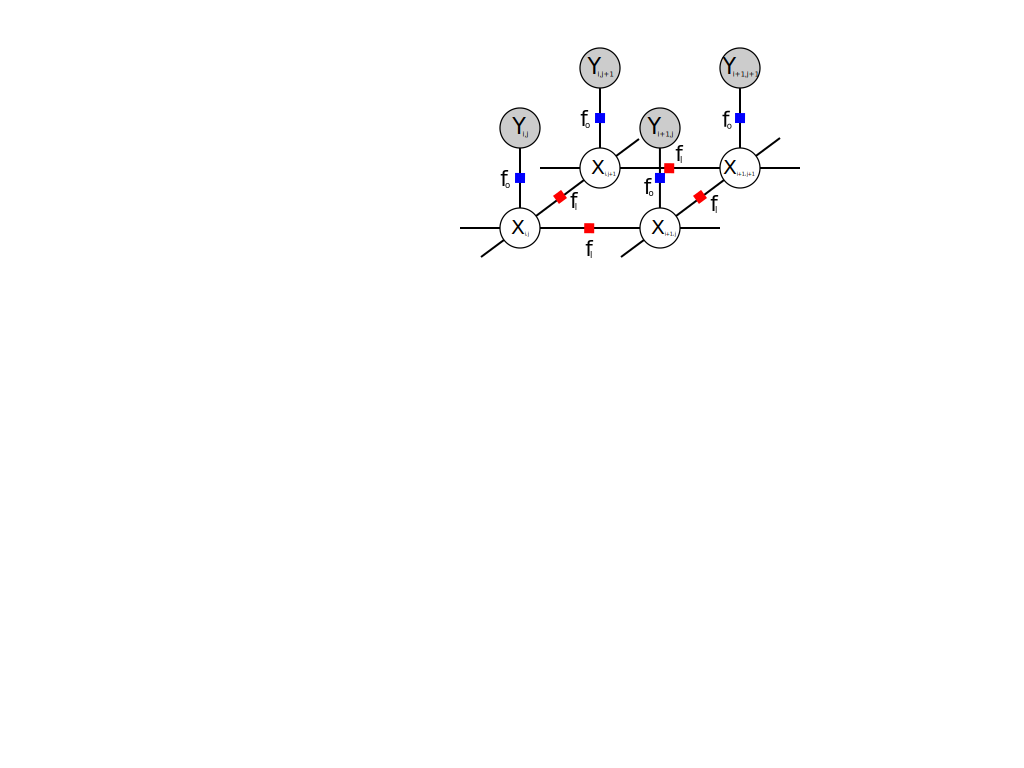
\includegraphics[width=5cm]{phase_fg_frey.pdf}
    \end{column}
    \begin{column}{5cm}
      \begin{itemize}
      \item $Y_{(i, j)} \in \mathbb{R}$ (continuous!) 
      \item $x_{(i, j)} \in [0, 2\pi)$ (continuous!) 
      \end{itemize}
    \end{column}
  \end{columns}
  
  
  \begin{columns}
    \begin{column}{5cm}
      \begin{block}{Observation Potential}
        $f_o = \delta ((Y_{(i, j)} mod 2\pi) - X_{(i, j)})$
      \end{block}
    \end{column}

    \begin{column}{5cm}
      \begin{block}{Latent potential} 
        $f_l(X_1, X_2) = (X_1 - X_2)^2$
      \end{block}
    \end{column}
    
  \end{columns}
  
\end{frame}

\begin{frame}
  \frametitle{Discrete latent state, homogeneous factors}
  \begin{columns}
    \begin{column}{5cm}
      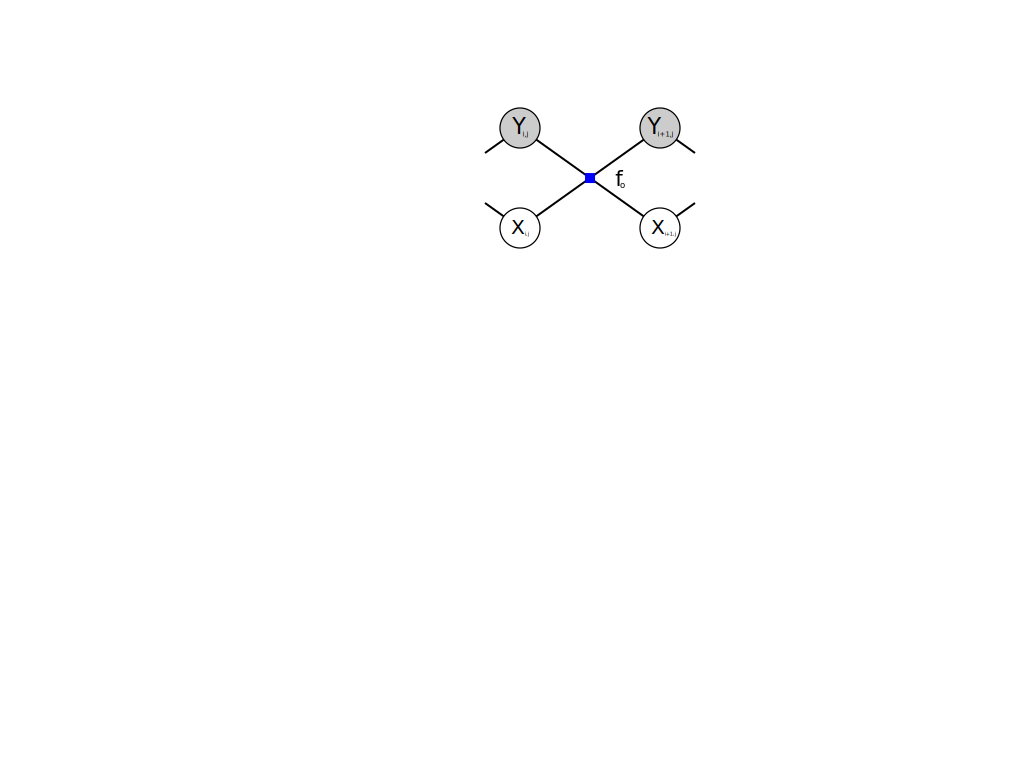
\includegraphics[width=5cm]{phase_fg_uniform.pdf}
    \end{column}
    \begin{column}{5cm}
      \begin{itemize}
      \item $Y_{(i, j)} \in \mathbb{R}$
      \item $x_{(i, j)} \in [1 ... K]$
      \end{itemize}
    \end{column}
  \end{columns}
  
  
%   \begin{columns}
%     \begin{column}{5cm}
%       \begin{block}{Observation Potential}
%         $f_o = \delta ((Y_{(i, j)} mod 2\pi) - X_{(i, j)})$
%       \end{block}
%     \end{column}

%     \begin{column}{5cm}
%       \begin{block}{Latent potential} 
%         $f_l(X_1, X_2) = (X_1 - X_2)^2$
%       \end{block}
%     \end{column}
    
%   \end{columns}


\end{frame}
  
\begin{frame}
  \frametitle{Discrete latent state, unique factors}
  I reformulated the problem to make inference easier. 
  
  \begin{columns}
    \begin{column}{5cm}
      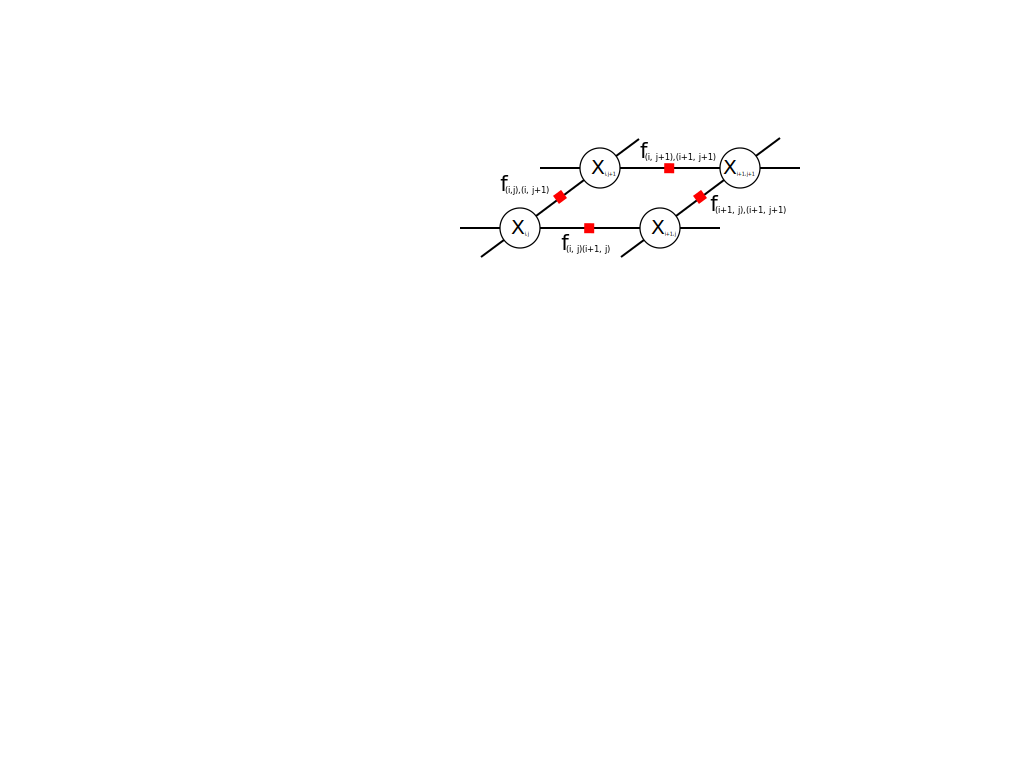
\includegraphics[width=5cm]{phase_fg_unique.pdf}
    \end{column}
    \begin{column}{5cm}
      \begin{itemize}
      \item $x_{(i, j)} \in [1 ... K]$
      \end{itemize}
    \end{column}
  \end{columns}
  
  \begin{block}{Unique (non-homogeneous) factors} 
    Every two adjacent $X_i, X_j$ on the lattice have a unique factor
    between them that incorporates the information from the data. 
  \end{block}
\end{frame} 

\section{Inference in MRFs}
\frame{\tableofcontents[currentsection]}

\begin{frame}
  \frametitle{Inference in MRFs}
  \begin{itemize}
  \item The MRF tells us how to compute $P(X, Y)$.
  \item Bayes rule  tells us how to compute $P(X | Y)$.
  \end{itemize}
  
  \begin{block}{Bayes Rule} 
    \begin{equation*}
      P(X | Y ) = \frac{P(Y | X) P(X)}{\sum_XP(Y|X)P(X)} \propto P(Y | X) \cdot  P(X) = P(X, Y)
    \end{equation*}
  \end{block}

  \pause
  Note: taking the above sum is hard! 
  
  There are some generic approaches to get around this: 
  \begin{itemize}[<+->]
  \item Traditional numerical integration
  \item optimize to find MAP solution
  \item Solve a similar, easier problem and perturb (variational methods)
  \item draw samples from $p(X | Y)$ to empirically estimate posterior
  \end{itemize}
  
\end{frame}

\begin{frame}
  \frametitle{Markov-Chain Monte Carlo}
  Markov Property: next state only depends on current state
  \begin{equation*}
    p(x_{t+1} | x_{1:t}) = p(x_{t+1} | x_{t})
  \end{equation*}
  
  \begin{block}{Main idea}
    Construct a Markov chain with the equilibrium distribution equal to your target distribution
  \end{block}
  Used in situations where you want to sample from
  $\pi(x)$ but only can compute $\pi^\ast(x) = Z \pi(x)$, $Z$ unknown. 

  \textit{But how do we construct a chain with equilibrium distribution $\pi(x)$?}
\end{frame}

\begin{frame}
  \frametitle{Metropolis-Hastings (1953) }
  Simple idea: randomly propose new location in state space, 
    sometimes go there! (From statistical physics   \cite{Metropolis_Equation_1953})
  \begin{columns}
    \begin{column}{5cm}
      
      We use a proposal distribution, $q(x \rightarrow x^\ast)$ 
      Draw $x^\ast$ as a \textit{new target state} from this distribution. 
      \begin{equation*}
        x^\ast  \sim q(x^\ast | x)
      \end{equation*}
      
      We compute the ``Acceptance'' ratio :       
      \begin{equation*}
        a = \min (1, \frac{p(x^\ast)}{p(x)} \cdot 
        \frac{q(x \rightarrow x^\ast)}{q(x^\ast \rightarrow x)})
      \end{equation*}
    \end{column}

  \begin{column}{5cm}
    \includegraphics[width=5cm]{notmine/Bishop_Figure11-9}
    \end{column}
  \end{columns}

\end{frame}

\begin{frame}
  \frametitle{Gibbs Sampling (1990) }
  \begin{columns}
    \begin{column}{5cm}
      If we can sample from conditional distributions, we can 
      use a more intelligent form of MH known as Gibbs Sampling  \cite{Geman_Stochastic_1990}
      \pause
      \begin{alertblock}{Requirements}
        To use Gibbs sampling on state variable $x_i$ we must be able
        to draw samples from $x_i \sim p(x_i | \{x_{j \neq i}\})$
      \end{alertblock}
    \end{column}
    
    \begin{column}{5cm}
      \includegraphics[width=5cm]{notmine/Bishop_Figure11-11}

      From Christopher Bishop. 
    \end{column}
  \end{columns}

\end{frame}


\begin{frame}
  \frametitle{Parallel Tempering (1991) } 
  (aka ``Replica Exchange Monte Carlo'' \cite{Swendsen_Replica_1986}, aka ``Something to do with your 8 cores'')
  \begin{itemize}
  \item Run N replicas of your chain, each at a different temperature
  \item Periodically propose MH-style swaps between adjacent chains
  \item Let's hot chains move around in flatter energy landscape
  \end{itemize}
  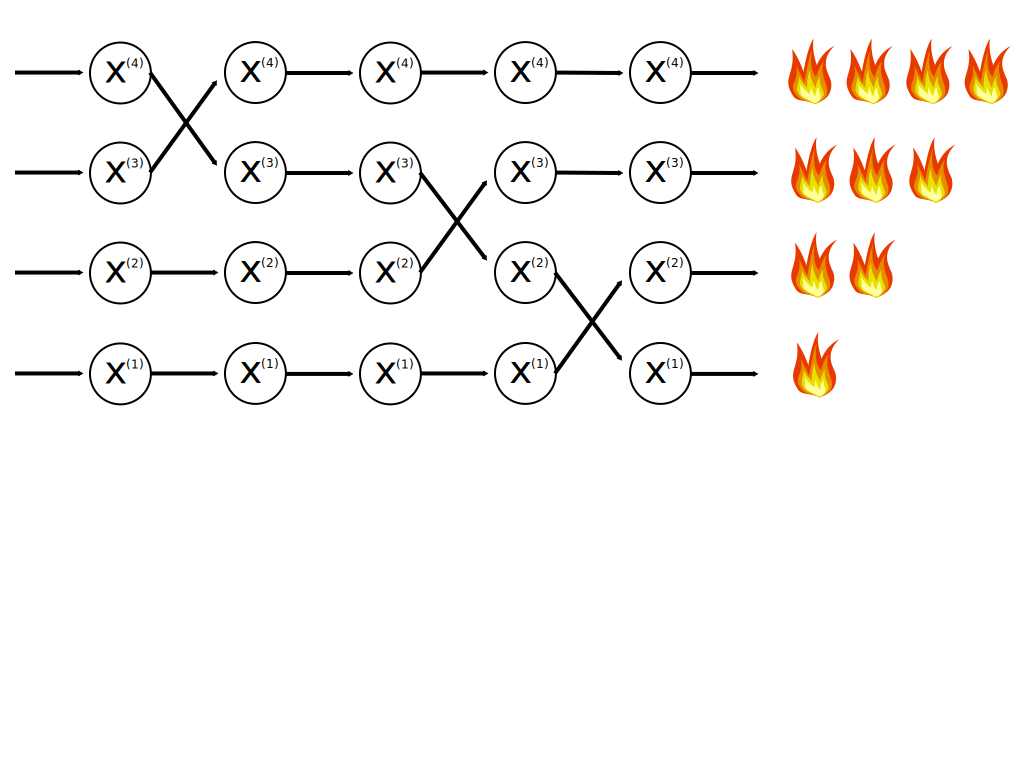
\includegraphics[width=8cm]{parallel_temp_fig.pdf}
\end{frame}

\begin{frame}
  \frametitle{Partial Replica Exchange (2000)}
  (aka ``Evolutionary MCMC'' \cite{Liang_Evolutionary_2000} aka ``Return of the GA'')
  \begin{itemize}
  \item Run N replicas of your chain, each at a different temperature
  \item Periodically propose MH-style swaps between \textbf{substates} in adjacent chains
  \item Let's hot chains move around in flatter energy landscape, but \textbf{lets better partial solutions move to cold chain}
  \end{itemize}
  \includegraphics[width=9cm]{partial_replica.pdf}
  
\end{frame}

\begin{frame}
  \frametitle{Data-driven MCMC (2002)}
  \begin{itemize}
    \item Any ``move'' is valid as long as it is reversible.  
    \item We can cheat a little bit and construct moves based on the data to help the chains mix, 
      without changing the target distribution
  \end{itemize}
  
  Zhuowen and Tu \cite{zhuowen_tu_image_2002} would pre-segment images
  with a heuristic and then use those segments as an MCMC proposal
  distribution.

\end{frame}

\begin{frame}
  \frametitle{Data-driven Partial Replica Exchange (2009)}
  \begin{columns}
    \begin{column}{6cm}
      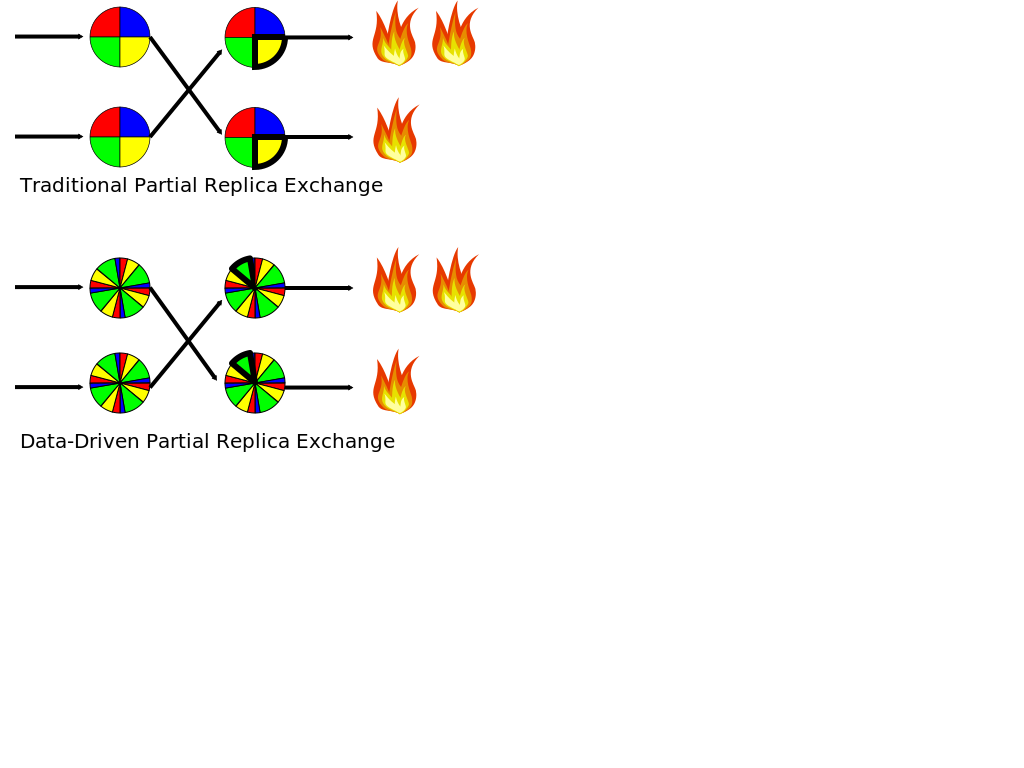
\includegraphics[width=7cm]{my_partial}
    \end{column}
    
    \begin{column}{4cm}
      \begin{itemize}[<+->]
      \item I just invented it! 
      \item Well, okay, I glued together two existing methods. 
      \end{itemize}
      \pause
      \begin{block}{This is the power of MCMC}
        Transition kernels (moves) nicely compose. 
      \end{block}
    \end{column}
  \end{columns}
\end{frame}
  
\begin{frame}
  \frametitle{MRFs and Parallelism}
  The conditional independence assumptions allow fine-grained parallelism
  
\end{frame}

\section{Results}
\frame{\tableofcontents[currentsection]}

\begin{frame}
  \frametitle{Our Implementation}
  \begin{itemize}
  \item Multi-threaded C++ engine, scales to 8 cores
  \item Python wrapper for GUI, vis, control, parameter tuning, 
  \end{itemize}
  
  \pause
  \begin{block}{Try it out}
    Source and presentation available for download on github
    \url{https://github.com/ericmjonas/mrimrf/}
  \end{block}

\end{frame}

\subsection{Synthetic Data}
\begin{frame}
  \frametitle{2-D Synthetic Data : The Sphere}
  \begin{columns}
    \begin{column}{3cm}
      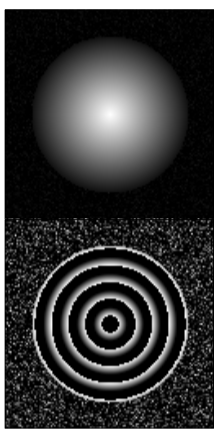
\includegraphics[width=3cm]{sphere2_128_image}
    \end{column}
    
    \begin{column}{8cm}
      \only<1> {
        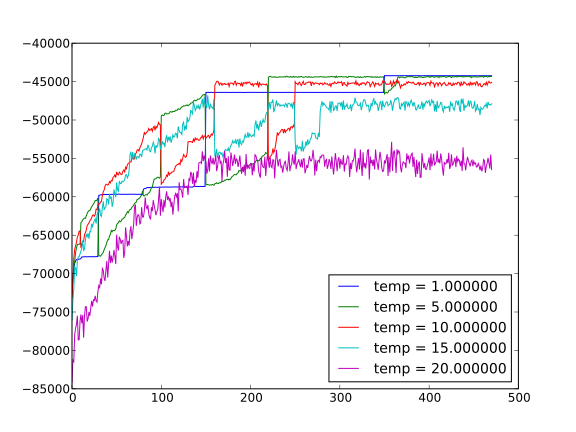
\includegraphics[width=8cm]{sphere2_128_all_loglikelihood}
      }
      \only<2> {
        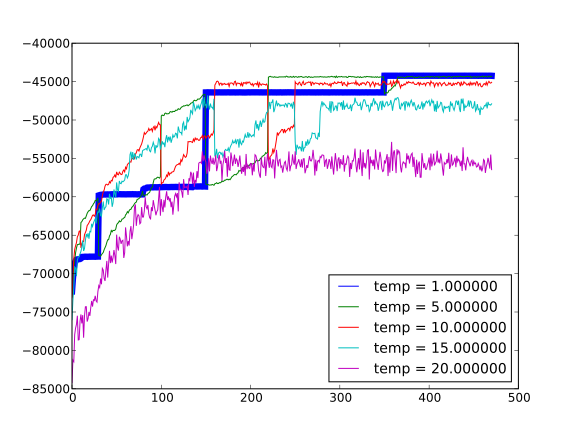
\includegraphics[width=8cm]{sphere2_128_all_loglikelihood_highlight}
      }
    \end{column}
  \end{columns}

\end{frame}

\begin{frame}
  \frametitle{2-D Synthetic Data : The Sphere : PT exchange}
  \only<1> {
    \includegraphics[width=6cm]{sphere_replica}
  }
  \only<2> {
    \includegraphics[width=9.5cm]{sphere_replica_zoom}
  }
\end{frame}

\subsection{Actual Data}

\begin{frame}
  \frametitle{Scores from run}
  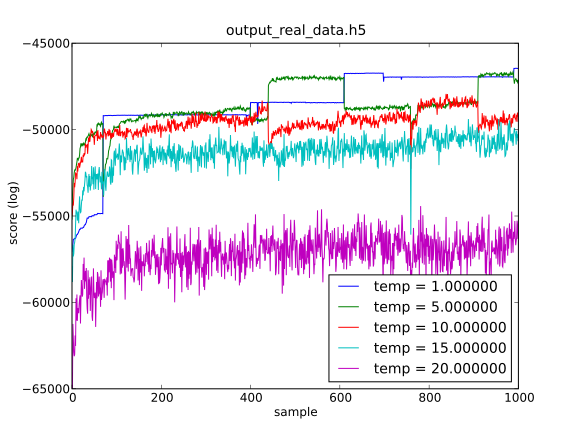
\includegraphics[width=10cm]{data_scores}
\end{frame}

\begin{frame}
  \frametitle{Chains over time}
  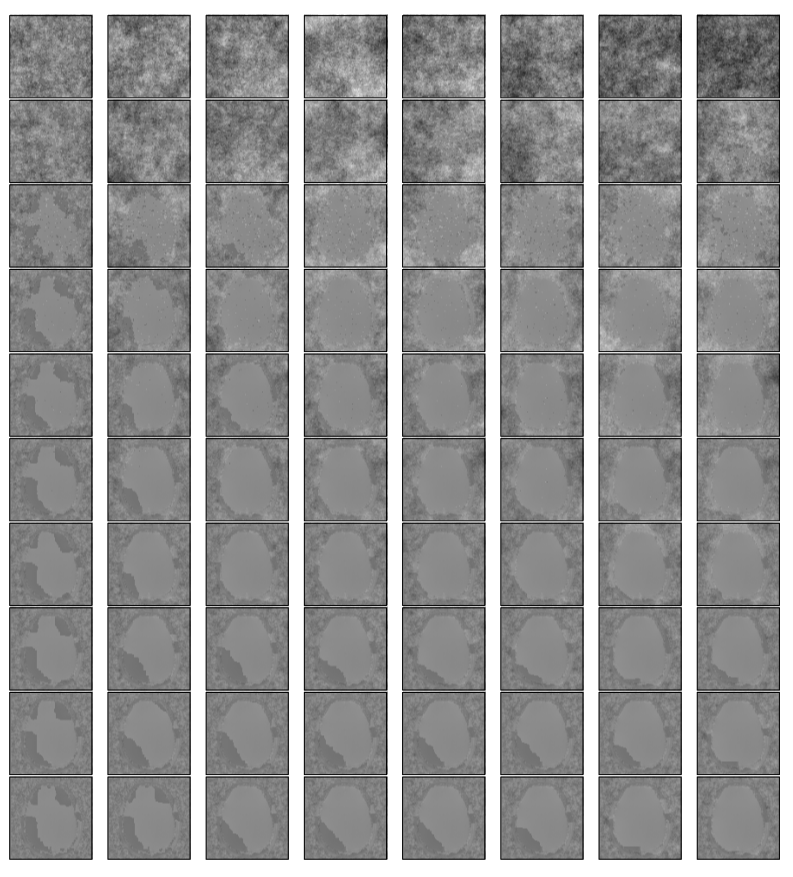
\includegraphics[width=8cm]{data_replicas}
\end{frame}

\begin{frame}
  \frametitle{Final Sample from Cold Chain}
  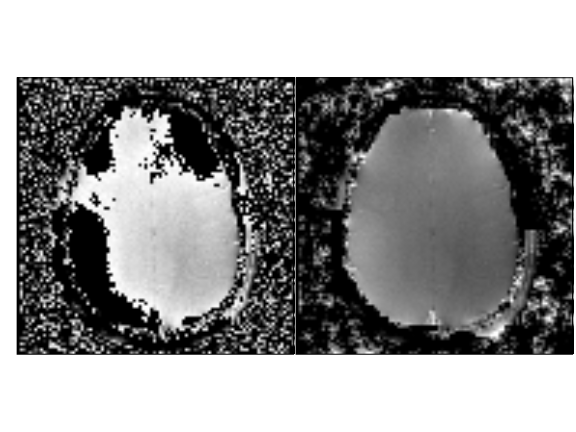
\includegraphics[width=10cm]{data_results}
\end{frame}

\section{Conclusion and Future Directions}
\frame{\tableofcontents[currentsection]}

\begin{frame}
  \frametitle{Why, man, why?}
  Why go through all this effort for mediocre performance? 
  \begin{itemize}[<+->]
    \item Why be Bayesian?  
       - incorporate prior information explicitly
       - probabilistic models compose
    \item Why use MCMC? 
       - MCMC ``black boxes'' often do the right thing with minimal work
       - Kernels compose nicely \cite{Bonawitz_Composable_2008}
    \item Why use factor graphs? 
       - reasonable prior expressing local dependence 
       - factors allow programmatic evaluation of conditional independencies, 
       thus can easily identify opportunities for parallelism
  \end{itemize}
  
\end{frame}

\begin{frame}
  \frametitle{Where to now?}
  \begin{itemize}[<+->]
  \item Exact sampling using Systematic Stochastic Search \cite{Mansinghka_Systematic_2008}
  \item Better neighborhood connectivity
  \item Better data likelihood
  \item GPU implementation -- CUDA makes this easy 
  \item Better visualization of posterior?
  \item Reconstruction? 
  \end{itemize}
\end{frame}

\begin{frame}
  \frametitle{More information}
  \begin{block}{Try it out}
    Source and presentation available for download on github
    \url{https://github.com/ericmjonas/mrimrf/}
  \end{block}

  \pause
  Questions? 

\end{frame}

\bibliographystyle{plain}

\begin{frame}[allowframebreaks]{References}
\bibliography{mrimrf.bib}
\end{frame} 

\end{document}
